\section{Hardware}
This section details the hardware components and implementation of Pookie, illustrating the as-is design and the current design. Overall, the design concept has been finalized, and the team is working towards assembling and integrating all components. 

\subsection{Hardware Overview}
The 3D model of Pookie was created using Fusion 360, featuring a compact and interactive design. Initially, the design had a fully rounded head with a curved LED display, as shown in the earlier prototype in Figure \ref{fig:initial}. This design was akin to many referenced desktop robots, with a dynamic and engaging physical appearance. However, this was later modified because the LED screen is flat and does not conform to a curved surface. To accommodate this, the updated design features a more rectangular head with a flat front panel, ensuring proper integration of the LED display while still maintaining an anthropomorphic design. 

\begin{figure}[ht]
    \centering
    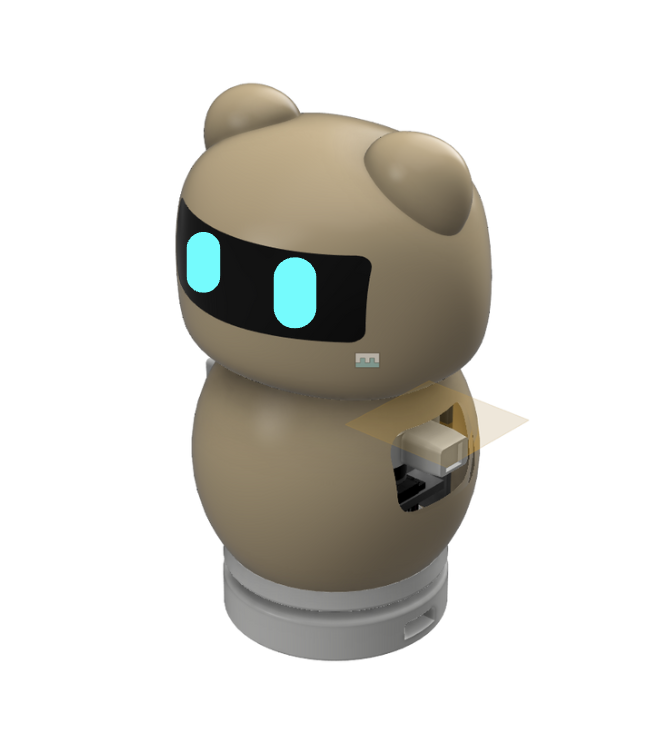
\includegraphics[width=0.52\textwidth]{initial.png}
    \caption{Initial Design of Pookie}
    \label{fig:initial}
\end{figure}

Pookie’s LED display serves as its face, with illuminated eyes that create an engaging and friendly expression. Positioned above the display is a camera. Designed with a modularity concept, Pookie’s head and hands are detachable, allowing easy access to internal hardware for maintenance or upgrades. The spherical arms are designed to be movable, enhancing its interactive capabilities. The base of the robot houses the Jetson Nano, along with speakers for audio output. 

The design choices focus on creating a friendly, interactive, and easily maintainable robot, ensuring that Pookie remains both functional and engaging for users. In particular, the revisions made in semester 2 include modularity. For instance, Pookie’s head is not just a spherical helmet, but rather two half-spheres that can be assembled and disassembled. Additionally, Pookie’s arms and neck are now connected using a neodymium magnet, further contributing to its modular design. 

\begin{figure}[ht]
    \centering
    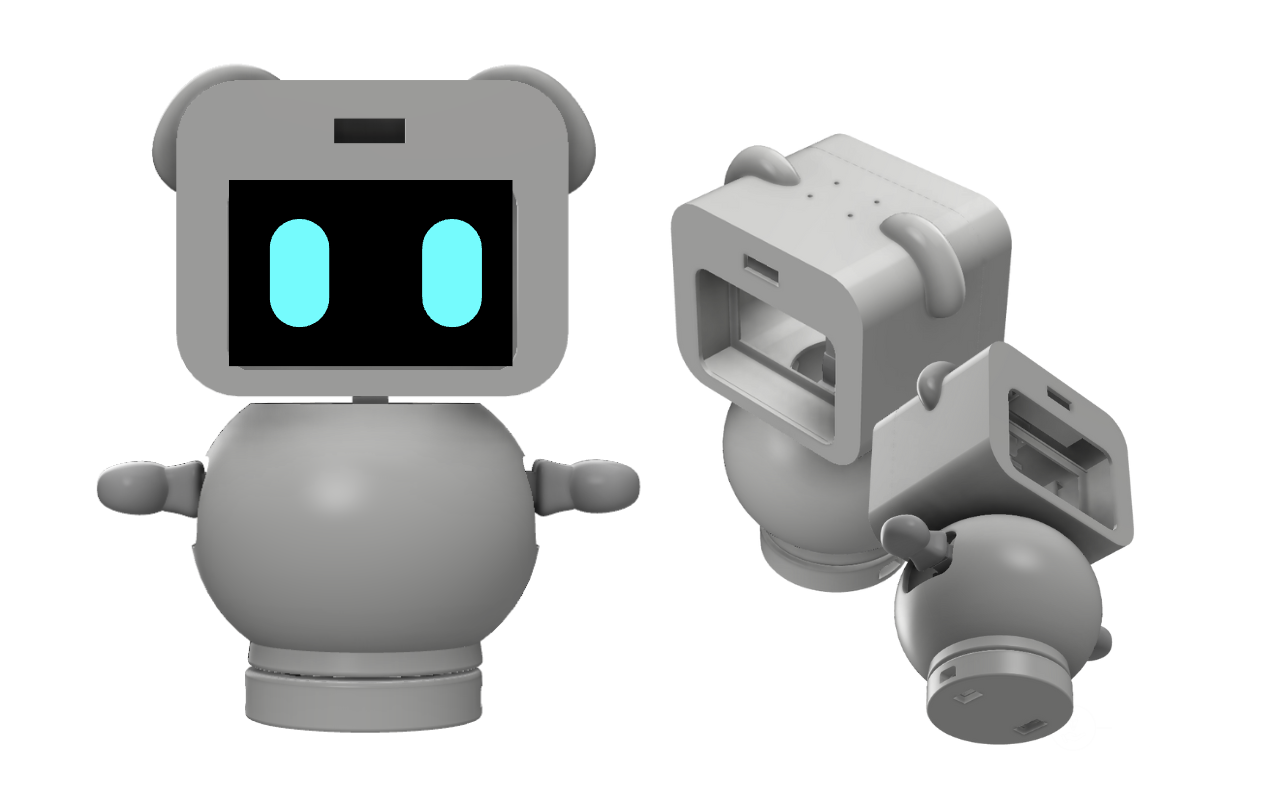
\includegraphics[width=0.85\textwidth]{new_des.png}
    \caption{Updated Design of Pookie}
    \label{fig:new_des}
\end{figure}

\newpage
Beneath the outer shell, Pookie's internal structure is designed to accommodate servo motors that control the movement of its head and arms by bevel gear mechanism allowing Pookie to perform simple gestures in a straightforward motion with four degrees of freedom. This is the as-is design, as shown in Figure \ref{fig:new_des}.

\begin{figure}[!ht]
    \centering
    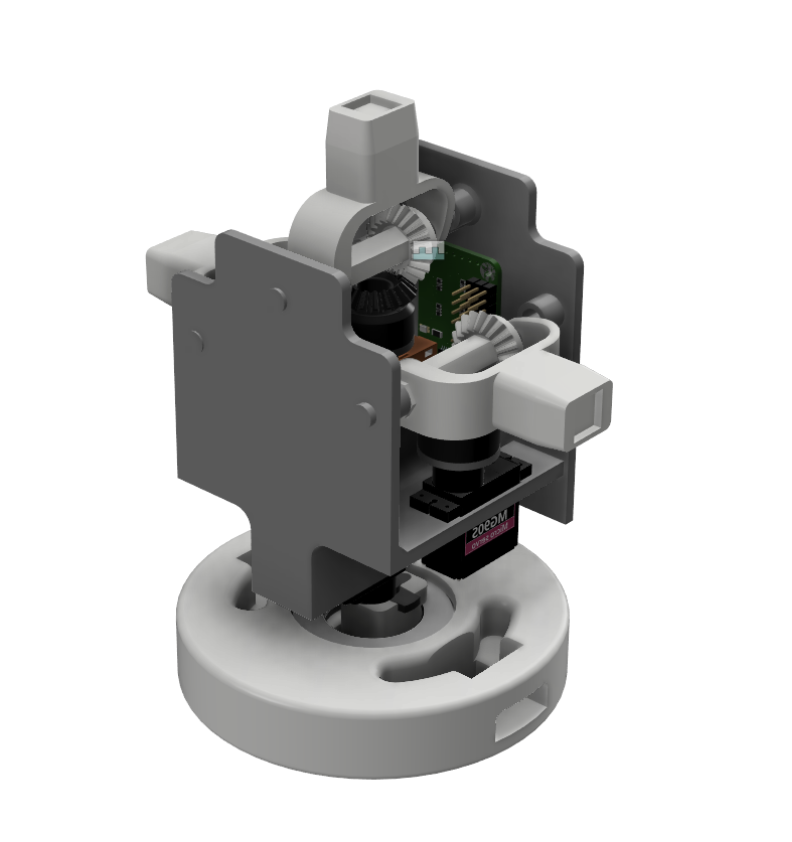
\includegraphics[width=0.6\textwidth]{internal.png}
    \caption{Internal Structure Design of Pookie}
    \label{fig:internal}
\end{figure}

Currently, several components of Pookie, including its head, motor brackets, gear, and other internal elements, have been 3D printed. Similarly, the hardware components necessary for assembly have almost all been acquired, missing only the speakers, which are rather hard to find. 

\subsection{Hardware Challenges}
One of the challenges encountered during the development process was ensuring that all 3D-printed components fit together properly. Some initial prints had slight misalignments, requiring adjustments to the design to achieve a more precise fit. These refinements helped improve the overall assembly process and ensure better compatibility between components.

Another challenge faced during the printing process was the size of each component, which was designed with flexibility in space in mind. This resulted in relatively large parts that could not fit in 3D printers. The solution was to break the parts into smaller pieces and construct them into one larger whole.
